% !TEX root = thesis.tex

% Front cover
% 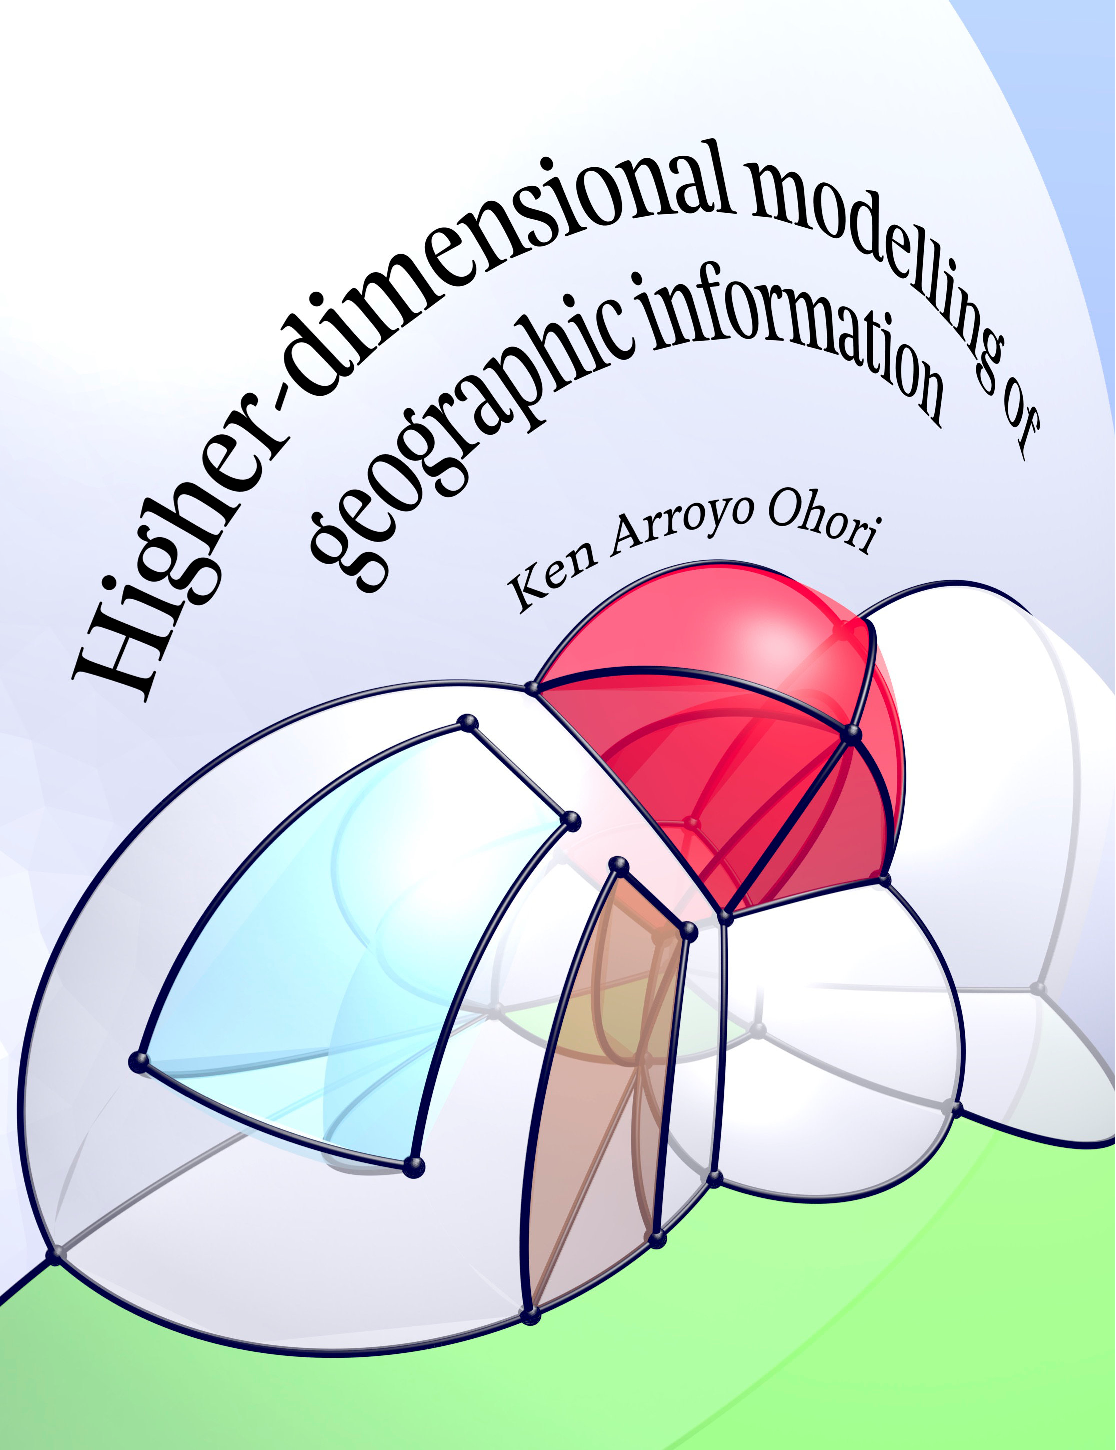
\includepdf{cover-front.pdf}

% Half-title
\author{Ken Arroyo Ohori}
\title{Higher-dimensional modelling of geographic information}
\date{}
\maketitle

% Copyright page
\clearpage
\thispagestyle{empty}
\null%
\label{thesis:colophon}
\vfill
\pdfbookmark[1]{Colophon}{thesis:colophon}
Written in 2014--2016 by
{\makeatletter
\href{http://ken.mx}{\@author}%
\makeatother}.

\cczero\ This work is released into the public domain using the CC0 code.

To the extent possible under law, the author has waived all copyright and related or neighbouring rights to this work.

To view a copy of the CC0 code, visit: \\
\url{http://creativecommons.org/publicdomain/zero/1.0/}

This thesis was typeset with \XeTeX\ 3.14159265--2.6--0.99992 (\TeX\ Live 2015) using the \mbox{{\fanciestfont{}Feijoa}}, \texttt{GT Pressura} and $\mathrm{Asana\ Math}$ typefaces.
Most of the figures were created using OmniGraffle, Affinity Designer or Blender, often with the help of \LaTeX{}\textsuperscript{i}T.

The source code of this thesis is available at: \\
\url{https://github.com/kenohori/thesis}

\textbf{Cover}: \\
Model of a 4D house represented as a 4D cell complex.
The cells of the model were manually defined and embedded in $\mathbb{R}^4$, projected inwards/outwards to the volume of a 3-sphere ($S^3$), stereographically projected to $\mathbb{R}^3$ and exported as an\ {}.obj file.
This was then imported in Blender and rendered using a perspective projection down to 2D.
See \refse{se:4dto3d} for more details.

% Official title
\begin{titlepage}
\null%
\label{thesis:title}
\vspace{3em}%
\pdfbookmark[1]{Title}{thesis:title}
\begin{center}

%% Skip space as in half-title
\vspace*{4\baselineskip}

%% Print the title.
{\makeatletter
\fanciestfont\huge\@title%
\makeatother}
\vfill

%% Apart from the names and dates, the following text is dictated by the
%% promotieregelement.

{\Large Proefschrift}

\medskip

{ter verkrijging van de graad van doctor \\
aan de Technische Universiteit Delft, \\
op gezag van de Rector Magnificus prof.~ir.~K.~C.~A.~M.~Luyben, \\
voorzitter van het College voor Promoties, \\
in het openbaar te verdedigen op \\
6 april 2016 om 12.30 uur}

\medskip

door

\medskip

%% Print the full name of the author.
\makeatletter
{\Large Gustavo Adolfo Ken {\scshape Arroyo Ohori}}
\makeatother

\medskip

Master of Science in Geomatics \\
geboren te Mexico-Stad, Mexico.

\end{center}
\end{titlepage}

% Official verso
\clearpage
\thispagestyle{empty}
\null%
\label{thesis:committee}
\vfill
\pdfbookmark[1]{Doctoral committee}{thesis:committee}

\noindent This dissertation has been approved by the

\medskip\noindent
\begin{tabular}{@{}ll@{}}
  \quad{}promotor: & Prof.\ dr.\ J.\ Stoter \\
  \quad{}copromotor: & Dr.\ H.\ Ledoux \\
\\
\multicolumn{2}{@{}l@{}}{Composition of the doctoral committee:} \\
\\
  \quad{}Rector Magnificus & chairperson \\
  \quad{}Prof.\ dr.\ J.\ Stoter & Delft University of Technology, promotor \\
  \quad{}Dr.\ H.\ Ledoux & Delft University of Technology, copromotor \\
\\
\multicolumn{2}{@{}l@{}}{Independent members:} \\
\\
  \quad{}Prof.\ dr.\ E.\ Eisemann & Delft University of Technology \\
  \quad{}Prof.\ dr.\ M.\ van\ Kreveld & Utrecht University \\
  \quad{}Dr.\ R.\ Lindenbergh & Delft University of Technology \\
  \quad{}Prof.\ dr.\ ir.\ A.\ van\ Timmeren & Delft University of Technology \\ 
\\
\multicolumn{2}{@{}l@{}}{Other member:} \\
\\
  \quad{}Dr.\ G.\ Damiand & Claude Bernard University Lyon 1 \\
\end{tabular}

This research was supported by the Dutch Technology Foundation STW, which is part of the Netherlands Organisation for Scientific Research (NWO), and which is partly funded by the Ministry of Economic Affairs (Project code: 11300).